%----------------------------------------------------------------------------------------
%	PACKAGES AND DOCUMENT CONFIGURATIONS
%----------------------------------------------------------------------------------------
\documentclass[11pt]{article}
\usepackage{amsmath} % Required for some math elements
\usepackage{hyperref} 
\usepackage{xcolor}
\usepackage{lipsum} 
\usepackage{cite}
\usepackage{graphicx} % Required for the inclusion of images
\usepackage{algorithmic}
\usepackage{array}
\usepackage{bookmark}
\usepackage{listings}
\usepackage{amssymb}
\usepackage{enumitem}
\usepackage{pythonhighlight}
\usepackage[T1]{fontenc}
\usepackage{inconsolata}
\usepackage[margin=8mm]{geometry}
\usepackage[caption=false, font=footnotesize]{subfig}
\usepackage{fancyhdr}
\pagestyle{fancy}
\renewcommand{\headrulewidth}{0.4pt}
\renewcommand{\footrulewidth}{0.4pt}

\usepackage[active,tightpage]{preview}
\renewcommand{\PreviewBorder}{1in}
\newcommand{\Newpage}{\end{preview}\begin{preview}}
  


\newlist{steps}{enumerate}{1}
\setlist[steps, 1]{label = Step \arabic*:}

\hypersetup{ %color attributes of citation, link, etc.
    colorlinks=true,
    linkcolor=blue,
    filecolor=gray,      
    urlcolor=blue,
    citecolor=blue,
}

\newcommand{\matlab}{\textsc{Matlab }} %very important and totally necessary addition
\newcommand{\hdotrule}[1]{\hbox to \textwidth{\leaders\hbox to #1pt{\hss . \hss}\hfil}}

\newcommand\Item[1][]{%
  \ifx\relax#1\relax  \item \else \item[#1] \fi
  \abovedisplayskip=0pt\abovedisplayshortskip=0pt~\vspace*{-\baselineskip}}
%----------------------------------------------------------------------------------------
%	DOCUMENT INFORMATION
%----------------------------------------------------------------------------------------

\title{ECEN 405 \\ Lab 3: Power converters \\ (Part 1 - Non-Synchronous buck converter) Submission}
\author{Daniel Eisen : 300447549}
\date{\today}

\begin{document}
\begin{preview}

    \maketitle
    \hrule
    %----------------------------------------------------------------------------------------
    %	DOCUMENT CONTENT
    %----------------------------------------------------------------------------------------
    \section{MOSFET Source}
    \begin{center}
        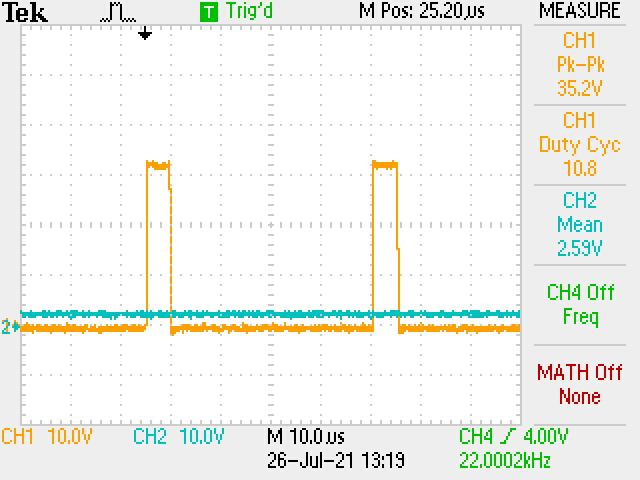
\includegraphics[width=0.33\textwidth]{img/D10_22K.JPG}
        \includegraphics[width=0.33\textwidth]{img/D80_22K.JPG}

        \textit{Continuous Mode Source and Output at $D \in \{0.1, 0.8\}$}
    \end{center}
    The waveform above shows was captured at the high-side FET's source and shows  the PWM signals (at 10\% and 80\%) scaled to the supply voltage (30V). Also present is the filter DC output.

    \section{Efficiency vs Output Current}
    \begin{center}
        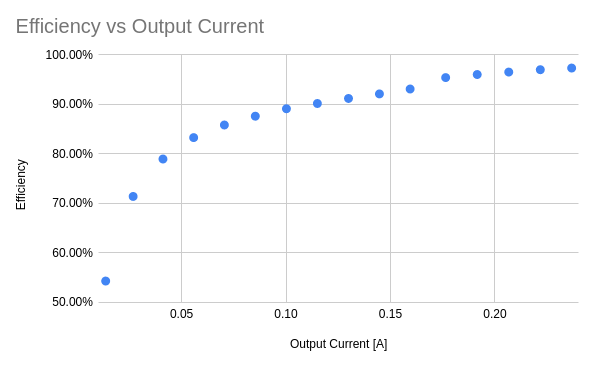
\includegraphics[width=0.33\textwidth]{img/nonsync_eff.png}
    
    \textit{Efficiency vs Output Current of Circuit (Collected via D sweep)}
    \end{center}

    The above figure shows the varying efficiency of the the buck converter with increasing output current. Observe that as the output current increases, the efficiency asymptotically increases towards its maximum. This is due to change in dominance between Switching and Conduction losses. At low duty cycles, conduction time and thus losses make up a small proportion of input current draw while the switching losses remain fixed (for a constant switching frequency and load). Ie for close to no output current, they always remain a lower limit on input current draw, and this proportion shift as D increases (and thus output current) and conduction losses make up the more of the proportion.

    \section{Synchronous vs Non-Synchronous Efficiency}
    \begin{center}
        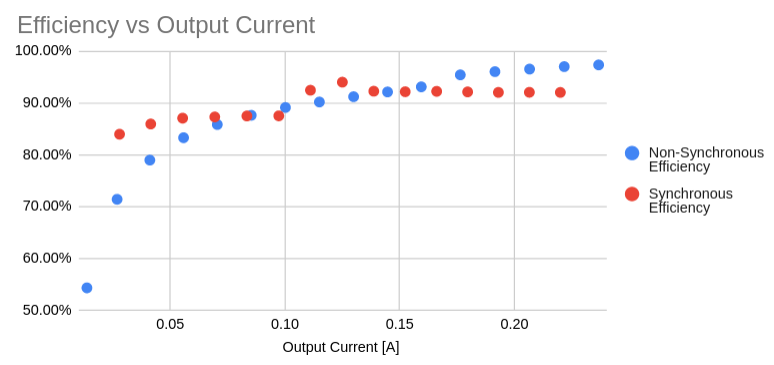
\includegraphics[width=0.33\textwidth]{img/eff_comp.png}
        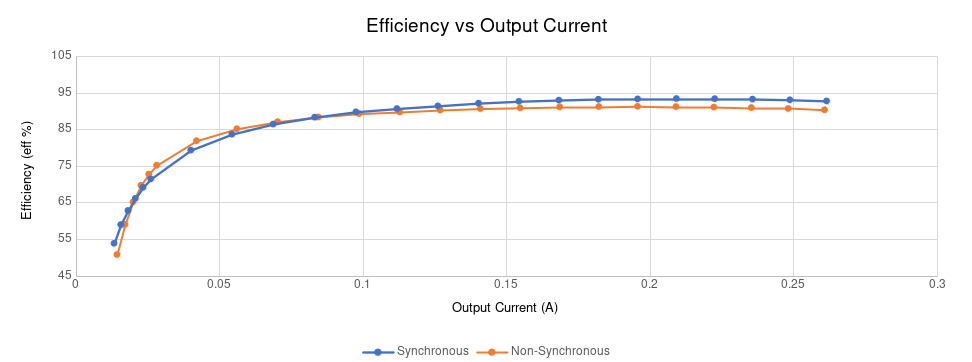
\includegraphics[width=0.33\textwidth]{img/sync_vs_non-sync.png}

    \textit{Efficiency vs Output Current Comparison between non-sync and sync \\(Left: Ours, Right: Niels/Nick to show what it should have looked like)}

    The key differences in efficiency between sync and non-sync topologies is the low end of output current the lower they are more similar in efficiency but as output current increases the higher losses in the diode take over and the difference in efficiency makes itself more apparent.
    
    Note due the very low max output currents these labs were running at, margin or error between the different circuit can result in erroneous results, as seen in left figure.

    \end{center}
    \section{Use-cases and Applications}

    \section{Reduced Switching Frequency}
    \begin{center}
        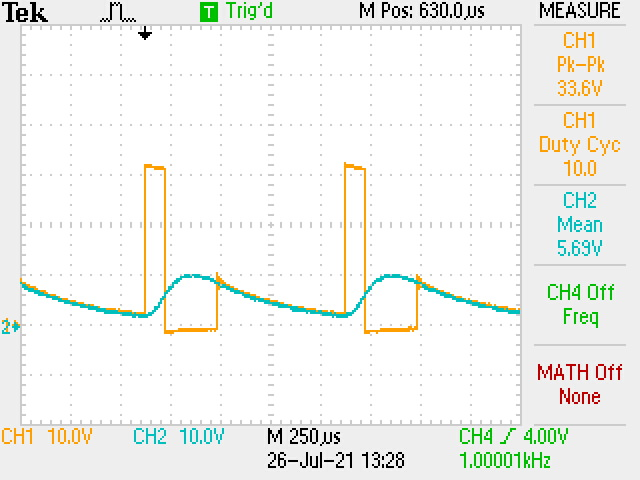
\includegraphics[width=0.33\textwidth]{img/D10_1K.JPG}
        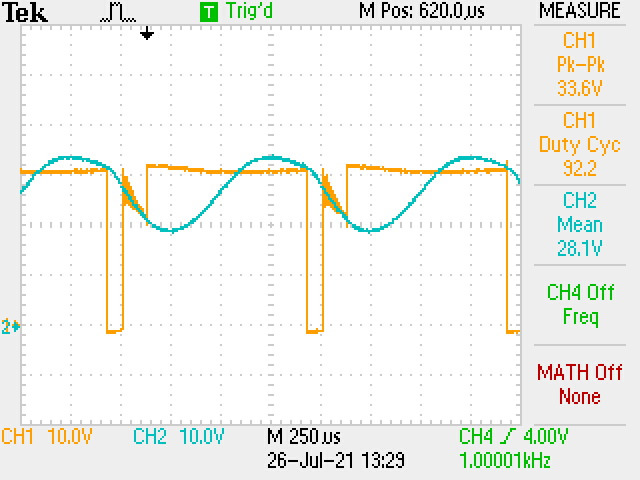
\includegraphics[width=0.33\textwidth]{img/D80_1K.JPG}

        \textit{Discontinuous Mode Source and Output at $D \in \{0.1, 0.8\}$}
    \end{center}

    THe above figures shows the buck-converter transitioned into discontinuous conduction mode. It is observed that the 10\% and 80\% PWM scaled output, but also a lower voltage decaying step part way into the high side off time. This is due the inductor current reaching zero.

    \hrule
\end{preview}
\end{document}